\section{Clustering}

\subsection{K-means Clustering (14 points)}

\begin{enumerate}

\item \textbf{(6 Points)}
Given $n$ observations $X_1^n = \{X_1, \dots, X_n\}$, $X_i \in \Xcal$, the K-means objective
is to find $k$
($<n$) centres $\mu_1^k = \{\mu_1, \dots, \mu_k\}$, and a rule $f:\Xcal \rightarrow
\{1,\dots, K\}$ so as to minimize the objective

\begin{equation}
J(\mu_1^K, f; X_1^n) = \sum_{i=1}^n \sum_{k=1}^K \indfone(f(X_i) = k) \|X_i - \mu_k\|^2
\label{eqn:kmeans}
\end{equation}

Let $\Jcal_K(X_1^n) = \min_{\mu^K, f} J(\mu_1^K, f; X_1^n)$. Prove that
$\Jcal_{K}(X_1^n)$ is a non-increasing function of $K$.

\begin{soln}

    We can easily see that $\Jcal_{K}(X_1^n)$ is a non-increasing function of $K$ by
    induction. For the base case, we have $\Jcal_{1}(X_1^n) = \sum_{i=1}^n \|X_i -
    \mu_1\|^2 $. For the inductive step, we have $\Jcal_{K+1}(X_1^n) = \min_{\mu_1^{K
    +1}, f} J(\mu_1^{K+1}, f; X_1^n)$ = $\min_{\mu_1^{K+1}, f} \sum_{i=1}^n \sum_{k=1}^
    {K+1} \indfone(f(X_i) = k) \|X_i - \mu_k\|^2 \leq \min_{\mu_1^{K}, f} \sum_{i=1}^n
    \sum_{k=1}^{K} \indfone(f(X_i) = k) \|X_i - \mu_k\|^2 = \min_{\mu_1^{K}, f} J(\mu_1^
    {K}, f; X_1^n) = \Jcal_{K}(X_1^n)$. Therefore, $\Jcal_{K}(X_1^n)$ is a
    non-increasing function of $K$.
    The less than or equal is hold since we can always set $\mu_1^{K+1} = \{\mu_1^{K},0\}$
    and keep the same $f$ to achieve $\Jcal_{K}(X_1^n)$. And by optimizing $\mu_{K+1}
    $, we can achieve $\Jcal_{K+1}(X_1^n)$ less than or equal to $\Jcal_{K}(X_1^n)$. 

\end{soln}

\item \textbf{(8 Points)}
Consider the K-means (Lloyd's) clustering algorithm we studied in class. We
terminate the algorithm when there are no changes to the objective.
Show that the algorithm terminates in a finite number of steps.

\begin{soln}
    First notice that for a given number of K, the possible choices of $\mu^k$ is finite. For each dimension of $\mu^k$, there are at most $\sum_{i=1}^{n} C_{n}^{i}=2^n$ possible centers. So the possible value of (1) is finite for a given dataset. \\
    And from the $t$ step to the $t+1$ step, the objective function is always decreasing unless it reach the optimal(since both the center calculation and regroup will result a decreasing in objective function unless no change).   
    Therefore, an algorithm optimize a finite valued function and grantee to decrease in each step until stop will terminate in a finite number of steps.
\end{soln}

\end{enumerate}



\subsection{Experiment (20 Points)}

In this question, we will evaluate
K-means clustering and GMM on a simple 2 dimensional problem.
First, create a two-dimensional synthetic dataset of 300 points by sampling 100 points each from the
three Gaussian distributions shown below:
\[
P_a = \Ncal\left(
\begin{bmatrix}
-1 \\ -1
\end{bmatrix},
\;
\sigma\begin{bmatrix}
2, &0.5 \\ 0.5, &1
\end{bmatrix}
\right),
\quad
P_b = \Ncal\left(
\begin{bmatrix}
1 \\ -1
\end{bmatrix},
\;
 \sigma\begin{bmatrix}
1, &-0.5 \\ -0.5, &2
\end{bmatrix}
\right),
\quad
P_c = \Ncal\left(
\begin{bmatrix}
0 \\ 1
\end{bmatrix},
\;
 \sigma\begin{bmatrix}
1 &0 \\ 0, &2
\end{bmatrix}
\right)
\]
Here, $\sigma$ is a parameter we will change to produce different datasets.

\begin{itemize}
\item First implement K-means clustering and the expectation maximization algorithm for GMMs.
Execute both methods on five synthetic datasets,
generated as shown above with $\sigma \in \{0.5, 1, 2, 4, 8\}$. Finally, evaluate both methods on \emph{(i)} the clustering objective~\eqref{eqn:kmeans} and \emph{(ii)}  the clustering accuracy. For each of the two criteria, plot the value achieved by each method against $\sigma$.

\item Both algorithms are only guaranteed to find only a local optimum so we recommend trying multiple
restarts and picking the one with the lowest objective value (This is~\eqref{eqn:kmeans} for K-means and the negative log likelihood for GMMs).
You may also experiment with a smart initialization
strategy (such as kmeans++).

\item
To plot the clustering accuracy,  you may treat the `label' of points generated from distribution
$P_u$ as $u$, where $u\in \{a, b, c\}$.
Assume that the cluster id $i$ returned by a method is $i\in \{1, 2, 3\}$.
Since clustering is an unsupervised learning problem, you should obtain the best possible mapping
from $\{1, 2, 3\}$ to $\{a, b, c\}$ to compute the clustering objective.
One way to do this is to compare the clustering centers returned by the method (centroids for
K-means, means for GMMs) and map them to the distribution with the closest mean.

\begin{soln}
    See Fig1.png and Fig2.png below.
    For code and data, please see hw5q1.ipynb.
    % insert two tables here, each table with 6 rows and 3 columns
    \begin{table}[h]
    \centering
    \begin{tabular}{|c|c|c|}
    \hline
    \textbf{Sigma} & \textbf{Accuracy} & \textbf{Objective} \\ \hline
    0.5 & 0.80 & 315 \\ \hline
    1 & 0.70 & 514 \\ \hline
    2 & 0.63 & 868 \\ \hline
    4 & 0.53 & 1623 \\ \hline
    8 & 0.50 & 3188 \\ \hline
    \end{tabular}
    \caption{K-means results}
    \label{tab:obj1}
    \end{table}
    \begin{table}[h]
    \centering
    \begin{tabular}{|c|c|c|}
    \hline
    \textbf{Sigma} & \textbf{Accuracy} & \textbf{Objective} \\ \hline
    0.5 & 0.65 & 550 \\ \hline
    1 & 0.56 & 891 \\ \hline
    2 & 0.50 & 1441 \\ \hline
    4 & 0.44 & 2950 \\ \hline
    8 & 0.40 & 6081 \\ \hline
    \end{tabular}
    \caption{EM results}
    \label{tab:obj2}
    \end{table}
    
% insert Fig1.png here
    \begin{figure}[h]
    \centering
    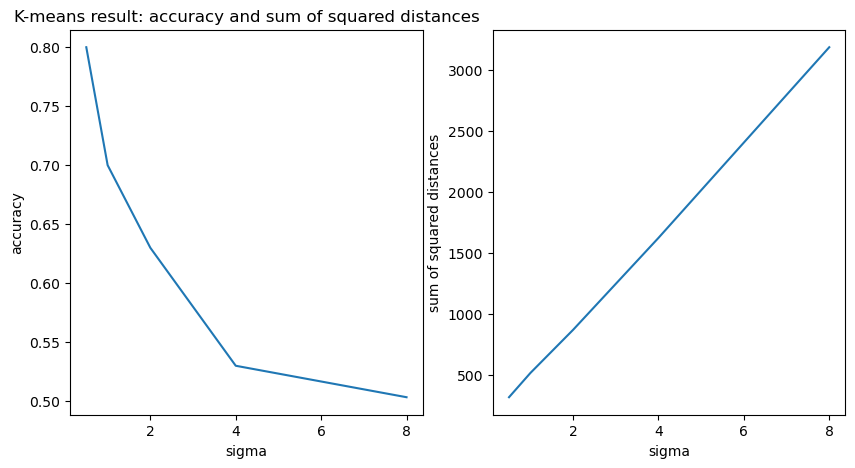
\includegraphics[width=0.8\textwidth]{Fig1.png}
    \caption{K-means result: accuracy and sum of squared distances}
    \label{fig:obj}
    \end{figure}
% insert Fig2.png here
    \begin{figure}[h]
    \centering
    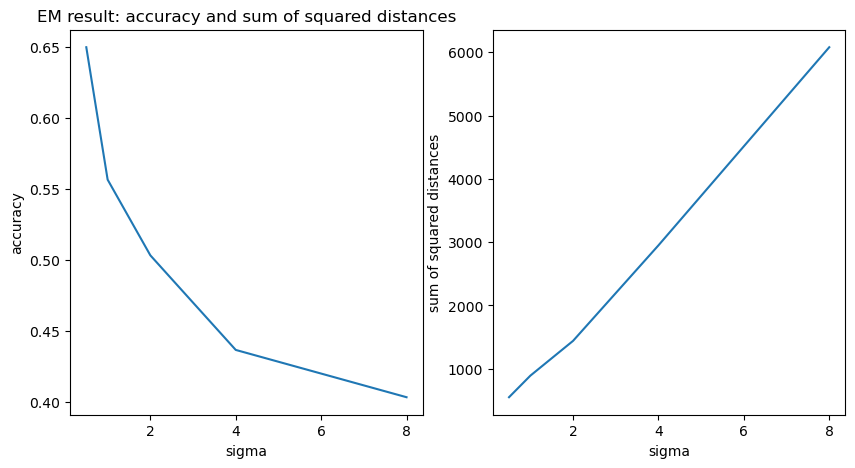
\includegraphics[width=0.8\textwidth]{Fig2.png}
    \caption{EM result: accuracy and negative log likelihood}
    \label{fig:obj}
    \end{figure}
\end{soln}

\end{itemize}

Points break down: 7 points each for implementation of each method, 6 points for reporting of
evaluation metrics.
